\documentclass[conference]{IEEEtran}
\IEEEoverridecommandlockouts
% The preceding line is only needed to identify funding in the first footnote. If that is unneeded, please comment it out.
%----------------------------------------------------------
\usepackage{cite}
\usepackage[pdftex]{graphicx}
% declare the path(s) where your graphic files are
\graphicspath{images/}
\DeclareGraphicsExtensions{.pdf,.jpeg,.png,.jpg}
\usepackage{amsmath,amssymb,amsfonts}
\usepackage{algorithmic}
\usepackage{graphicx}
\usepackage{textcomp}
\usepackage{array}
%\usepackage[caption=false,font=normalsize,labelfont=sf,textfon =sf]{subfig}
\usepackage{dblfloatfix}
\usepackage{url}
\usepackage{lipsum}
\usepackage{xcolor}
\usepackage{listings}

\def\BibTeX{{\rm B\kern-.05em{\sc i\kern-.025em b}\kern-.08em
    T\kern-.1667em\lower.7ex\hbox{E}\kern-.125emX}}
%----------------------------------------------------------
    \lstset{
        escapeinside={/*@}{@*/},
        language=Java,	
        basicstyle=\fontsize{8.5}{12}\selectfont,
        numbers=left,
        numbersep=2pt,    
        xleftmargin=2pt,
        frame=tb,
        columns=fullflexible,
        showstringspaces=false,
        tabsize=4,
        keepspaces=true,
        showtabs=false,
        showspaces=false,
        morekeywords={inline,public,class,private,protected,struct},
        captionpos=b,
        lineskip=-0.4em,
        aboveskip=10pt,
        extendedchars=true,
        breaklines=true,
        prebreak = \raisebox{0ex}[0ex][0ex]{\ensuremath{\hookleftarrow}},
        keywordstyle=\color[rgb]{0.5,0,0.35},
        commentstyle=\color[rgb]{0.25,0.5,0.35},
        stringstyle=\color[rgb]{red},
    }
%----------------------------------------------------------
\newcommand\largurafig{9cm}
\newcommand\recuodot{0.03cm}

\begin{document}

\title{Desenvolvimento do Jogo PONG com Processing3\\
{\footnotesize \textsuperscript{*} Sistemas Embarcados: Prof. Marco Reis - marco.reis@ba.docente.senai.brr}
}

% \author{\IEEEauthorblockN{Marco Reis, 41650-010\IEEEauthorrefmark{1}}
% \IEEEauthorblockA{\IEEEauthorrefmark{1}Robotics & Autonomous Systems Center,
% Senai Cimatec, Salvador, Brazil}% <-this % stops an unwanted space



\author{\IEEEauthorblockN{1\textsuperscript{st} Alexandre Adonai Gama da Silva}
\IEEEauthorblockA{
\textit{Senai - CIMATEC}\\
Salvador, Brasil \\
alexandre.s@aln.senaicimatec.edu.br}
\and
\IEEEauthorblockN{2\textsuperscript{nd} João Gabriel da Anunciação Calmon}
\IEEEauthorblockA{
\textit{Senai - CIMATEC}\\
Salvador, Brasil \\
joao.calmon@aln.senaicimatec.edu.br}
\and
\IEEEauthorblockN{3\textsuperscript{rd} João Vitor Silva Mendes}
\IEEEauthorblockA{
\textit{Senai - CIMATEC}\\
Salvador, Brasil \\
joao.mendes@aln.senaicimatec.edu.br}
}

\maketitle

\begin{abstract}
The present paper, aims to develop the classic game pong. The construction was done using the Processing platform, which, integrated with the Arduino IDE, made it possible to access and send the data, read by the Arduino UNO, from the Potentiometers and Pushbottons. However, the graphical interface was fully completed giving life to the famous Pong.
\end{abstract}

\begin{IEEEkeywords}
% Ver se vai deixar esse ou mudar
Processing, Arduino, Pong, Arduino IDE, Potentiometers, Pushbottons
\end{IEEEkeywords}

\section{Introdução}
O Pong é o primeiro jogo lucrativo da história em formato de vídeo. Criado por  Nolan Bushnell e Ted Dabney, o jogo se inspira no clássico jogo de tênis de dois jogadores em que as hastes/barras simulam as raquetes, e a bola da mesma forma que em uma partida de tênis, percorre a quadra até um dos jogadores não conseguir rebater\cite{TechTudo}. A versão clássica do PONG consiste em um console ligado a um monitor, sendo as hastes movidas por moedas. Nesta atividade, o objetivo é recriar o jogo buscando adicionar elementos gráficos e de \textit{gameplay} que a tecnologia contemporânea ao jogo não permitiria, porém respeitando a essência do jogo.

\section{Componentes Utilizados}
Esta seção se dedica a realizar uma breve apresentação de alguns dos principais componentes utilizados.

\subsection{Arduino UNO}
O microcontrolador Arduino (figura ~\ref{fig:arduino}) foi criado no ano de 2005 na Itália. A proposta por trás do produto era fornecer ao mercado,
em especial aos estudantes universitários, um microcontrolador versátil e de baixo custo. Atualmente existem disponíveis 
no mercado inúmeros modelos diferentes de Arduino, cada um com suas próprias peculiaridades, funcionalidades e nicho
aplicação.

Contudo, o que tais placas tem em comum é que são baseadas em um microprocessador de 8 
\textit{bits Atmel AVR reduced instruction set computer} 
(RISC), já que este permite que um conjunto de instruções pequenas e relativamente simples possam ter 
um tempo de execução aproximadamente constante \cite{evans2013arduino}. Ora, essa característica descreve 
muito bem um microcontrolador, já que o seu foco está no controle de sensores e atuadores através do processamento 
de quantidades pequenas de dados (se comparado a um processador).

Além das saídas de tensão e algumas portas de uso específico, o Arduino UNO conta com 14 portas digitais,
das quais 5 possuem a funcionalidade de PWM (recurso que permite a variação da tensão de saída de uma 
porta digital através da modulação por largura de pulso), e 6 portas analógica, que conforme será apresentado
mais adiante, podem ser usadas como saídas digitais. Ou seja, ele conta com um total de 19 portas de entrada e saída.

É válido ressaltar que o número de dispositivos acionados por ele pode ser ainda maior através do uso
da interface I2C ou alguns circuitos integrados que permitem o acionamento de inúmeros atuadores por 
meio de poucas portas do microcontrolador, como é o caso dos registradores de deslocamento, como por
exemplo o CI SN74HC595N.

\subsection{Pushbutton}
Os \textit{pushbutons}, também chamados de botões são componentes eletrônicos com os termineis elétricos separados por uma chave aberta, conforme a figura \ref{fig:pushbutton}. Ao ser pressionado estes contatos são fechados e a corrente elétrica pode fluir pelos seus terminais \cite{MasterWalkerPushButton}.

\subsection{Potenciômetro}
Um potenciômetro é um componente eletrônico que possui uma resistência interna e pode variar o valor de resistência entre os seus terminais conforme a rotação de um eixo. Esse eixo ao ser rotacionado  movimenta um contato elétrico e assim a resistência dos dois terminais da extremidade e o terminal central (movel) pode ser variada \cite{MasterWalkerPotenciometro}. Seu aspecto construtivo pode ser observado na figura \ref{fig:potenciometro}.

\begin{figure}[htbp]
\centerline{
    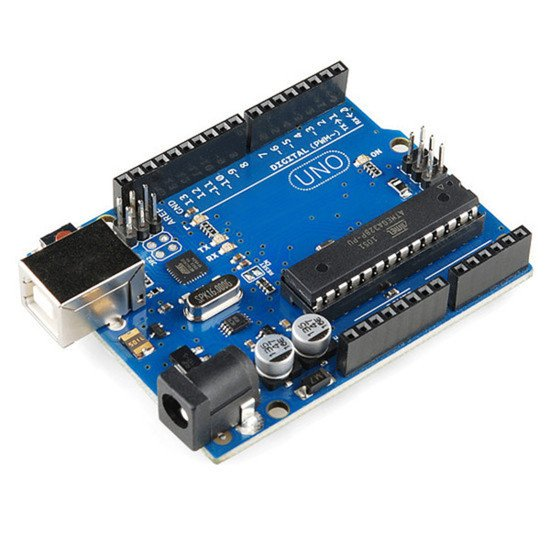
\includegraphics[width= 6cm]{images/arduino-uno.jpg}
    }
\caption{Arduino UNO.}
\label{fig:arduino}
\end{figure}

\begin{figure}[htbp]
\centerline{
    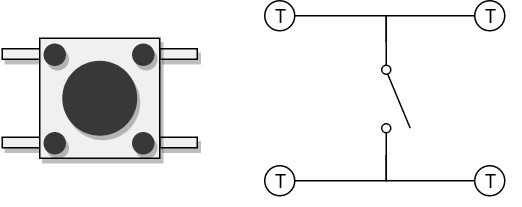
\includegraphics[width = 7cm]{images/Push-Button.jpg}
    }
\caption{Esquema elétrico de um pushbutton.}
\label{fig:pushbutton}
\end{figure}

\begin{figure}[htbp]
\centerline{
    \includegraphics[width = 6cm]{images/potenciômetro.png}
    }
\caption{Aspecto construtivo de um potenciômetro.}
\label{fig:potenciometro}
\end{figure}

\section{Esquematização do Circuito}
Para uma melhor didática de como foram feitas as conexões dos pontenciômetros e pushbottons ao arduino, foi demonstrado no Tinkecad \cite{Tinkercad} conforme a imagem ~\ref{fig:esquema}. As ligações dos potênciomentro foram, respectivamente, o terminal 1 ligado ao GND, o terminal 2 aos pinos analógicos A0 e A2 e o terminal 3 ligado ao 5V. Já os pushbottons, foram ligados, respectivamente, o terminal 1B aos pinos digitais 9 e 8 e o terminal 2B ao GND. 
\begin{figure}[htbp]
\centerline{
    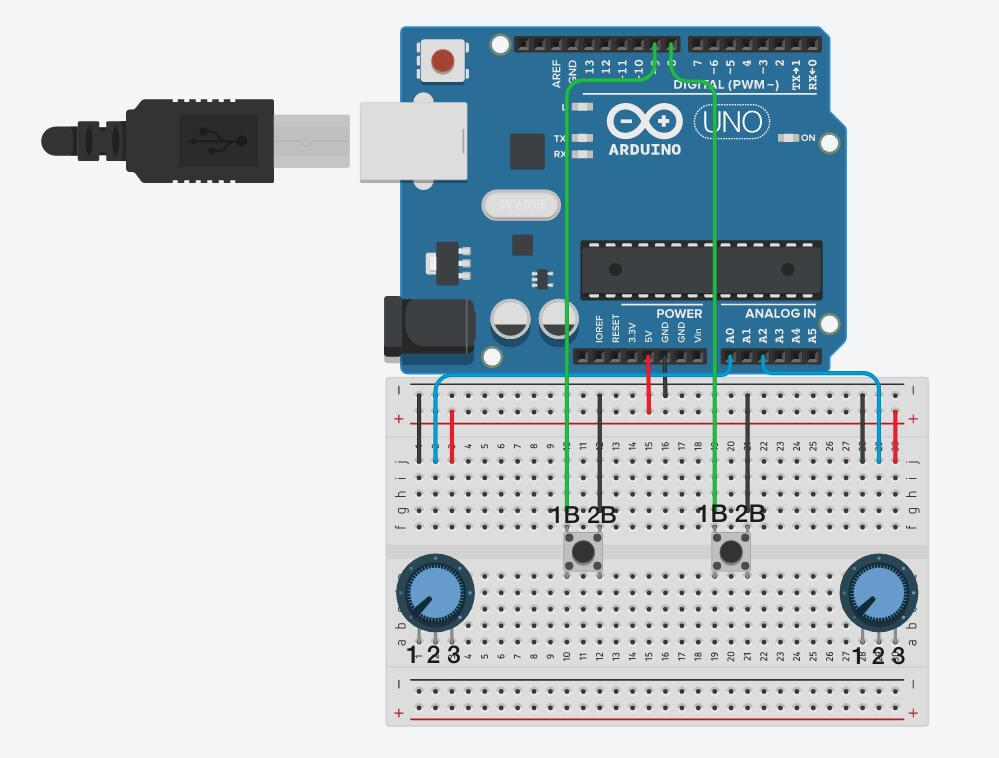
\includegraphics[width= 6cm]{images/Tinkercad.jpeg}
    }
\caption{Esquematização do Circuito.}
\label{fig:esquema}
\end{figure}
\section{Execução do projeto}

\subsection{Bola}\label{AA}
O código, representado abaixo, tem como objetivo criar a bola do jogo
e determinar sua trajetória, detectando os limites do campo e as duas 
hastes assim que se colidem, realizando o rebatimento. Primeiramente, 
foi declarado as funções fill, para determinar a cor da bola em RGB, 
e ellipse que cria a bola nas coordenadas x e y predeterminadas e a 
largura e altura também predeterminadas. Após isso, nas linhas 8 e 
9 é atribuido aos valores de x e y, eles mesmos somados as velocidade 
correspondentes, em que spx e spy são coordenadas que variam conforme
as condições posteriores(void draw) dando a sensação de movimento. Já mais abaixo, na linha 12 é determinado uma condição if, no qual limita a trajetória 
da bola de acordo com os limites superiores e inferiores do campo, 
realizando o rebatimento quando detectado. Na linha 17, há outro operador
if com condições para determinar se a bola colidiu com uma das hastes, dentro 
de seu bloco há mais dois operadores ternários, um if e um else, em que o if 
limita a váriavel bounce(rebatimento) em 7, no qual, nesse intervalo, a velocidade da bola será multiplicada por 1,3 e a função de rebatimento na haste e coloração da bola serão acionadas, após bounse igual ou maior que 7 o else será acionado e a velocidade e coloração da bola serão constantes, chamando somente a função de angulação.Nas linhas posteriores, é declarado a variável, onde a função check() é atribuída com o objetivo de verificar se a bola ainda está dentro do campo. Dessa forma se var for diferente de 0, chama-se a função score, e se var for igual a 1 ou 2 reseta-se a velocidade da bola. 
    \begin{lstlisting}
void ball() {
  
  fill(color_ball[0], color_ball[1], color_ball[2]);
  
  ellipse(x,y,size_ball,size_ball);
  
 
  x = x + sp_x;
  y = y + sp_y;

  
  if(y<10+size_ball/2 || y>height - (10+size_ball/2)){ 
  sp_y = -sp_y; 
      
  }
  
  if((sp_x<0 && x<10+width_bar+size_ball/2 && x>10+width_bar/2 && y>=pos_y_bar1-height_bar/2 && y<=pos_y_bar1 + height_bar/2) || (sp_x>0 && x>width-(10+width_bar+size_ball/2) && x<width-(10+width_bar/2) && y>=pos_y_bar2-height_bar/2 && y<=pos_y_bar2+height_bar/2)){
    if(bounce < 7){                                                    
      
      sp_x = sp_x * 1.3; 
      ball_spd_angular(sp_x, sp_y);
      bounce++;
      make_red_ball(30);
      
    }
    else{
      ball_spd_angular(sp_x, sp_y);
      }
  }
 
  int var = check();
  if(var != 0) score(var);
  
  if(var == 1 || var == 2){
     init_start = !init_start;
    }
}

    \end{lstlisting}


\subsection{Barras de Rebatimento}
A construção das barras de rebatimento e seu movimento é definido na função presente no código abaixo. Nas  duas primeiras linhas foi utilizado a função map(), que irá receber como argumento os respectivos parâmetros: a)valor do potenciômetro; b) Valor mínimo que do potenciômetro; c) valor máximo do potenciômetro, d) posição máximo que a barra pode assumir; e) posição mínima que a barra pode assumir. Se baseando na variação dos valores assumidos pelo potenciômetro, a função map irá retornar para as variáveis valor da posição de cada haste. Logo em seguida, é definido pela função rectMode(), o referência que as demais função irão utilizar para desenhar a barra, que neste caso será o centro. Por fim, são utilizadas as funções rect() que receberam como parâmetros o seguintes ítens: a) posição no eixo x; b) posição no eixo y; c)largura da barra, d)altura da barra; e) valor de referência para deixar as bordas arredondadas.
    \begin{lstlisting}
void bars_moviment(){
  pos_y_bar1 = map(pot_left, 0, 1023, 10 + height_bar/2, height-(10 + height_bar/2));
  pos_y_bar2 = map(pot_right, 0, 1023, 10 + height_bar/2, height-(10 + height_bar/2));
  rectMode(CENTER);
  pos_x_bar1 = 10 + width_bar;
  pos_x_bar2 = width - pos_x_bar1;
  rect(pos_x_bar1, pos_y_bar1, width_bar, height_bar, 50);
  rect(pos_x_bar2, pos_y_bar2, width_bar, height_bar, 50);
}
    \end{lstlisting}


\subsection{Comunicação Serial}
Para a realização da troca de dados entre o Arduino e o computador, mais especificamente o \emph{processing}, foi utilizado o cabo USB AB do Arduino, o mesmo empregado no processo de inscrição de novos códigos na placa. Quanto ao padrão de envio das informações, a mesma se deu de forma serial, ou seja, um bit é enviado após o outro de forma sequencial \cite{ArduinoHomepage}. Como haviam quatro informações que deveriam ser enviadas a cada ciclo, a saber a leitura analógica dos dois potenciômetros e a leitura digital dos dois \emph{pushbuttons}, foi preciso estabelecer um padrão de envio para que estes dados pudessem ser separados no momento da leitura. 

Para construção de um padrão de formatação das \emph{strings} o caractere '-' foi empregado como separador entre um valor inteiro e o outro, sempre escritos na mesma ordem, e finalizado pelo caractere de quebra de linha. O resultado obtido foram \emph{strings} no seguinte formato: "potenciômetro1 - potenciômetro2 - botão pause - botão reset \textbackslash n", no qual cada nome representa o valor lido em cada um dos componentes.

Em posse dessa configuração foi possível utilizar as funções \emph{readStringUntil()}, responsável por ler as informações da porta serial até o caractere informado como parâmetro ao método) e a \emph{split()}, responsável por separar uma \emph{string} em outras menores com base no parâmetro passado. Vale ressaltar que ambas são funções já implementadas no \emph{processing 3} \cite{ProcessingHomepage}.

\subsection{Sistema de Rebatimento}
Para criação do sistema de rebatimento, o qual deveria retornar a bola com uma angulação diferente a depender da região da barra atingida, foi tomado como base o valor do centro da barra na tela naquele instante (o mesmo valor usado para a sua movimentação) e a sua altura total, ou seja, um valor fixo. A fim de dividir a barra em oito seções de mesmo tamanho, conforme a figura ~\ref{fig:barra_dividida} foi considerado que a divisa entre elas estava a uma distância de um oitavo da altura da barra uma das outras e somando n/8 (com n variando de 1 a 4) ao valor da posição do centro da barra se obteve a divisão da parte superior e aplicando-se o mesmo procedimento, exceto pelo sinal oposto (subtração), foi possível realizar essa mesma operação para a as divisões abaixo do centro da barra.

\begin{figure}[htbp]
\centerline{
    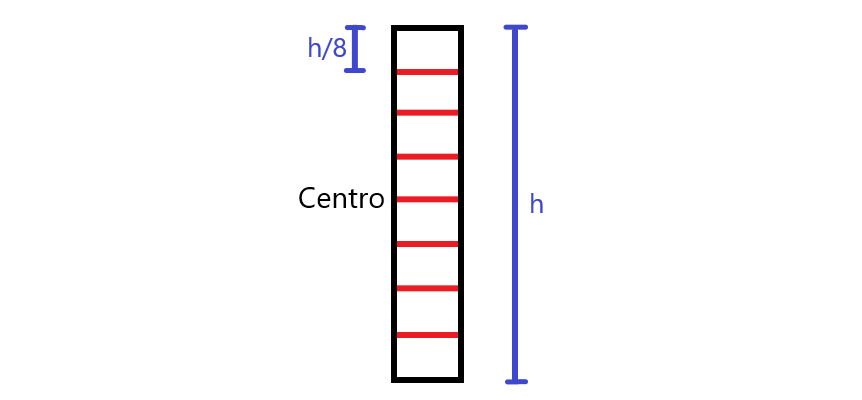
\includegraphics[width = \largurafig]{images/barra_dividida.png}
    }
\caption{Divisão das barras de rebatimento.}
\label{fig:barra_dividida}
\end{figure}

Durante o momento de encontro da bola com a barra, a fim de identificar a região de colisão, foi aplicada uma sequência de estruturas condicionais começando as verificações pelos dois seguimentos centrais, isto é, se a coordenada vertical da bola estava à uma distância menor ou igual a um oitavo do centro da barra, e então partindo gradualmente para aqueles que se encontravam a uma unidade de distância acima ou abaixo do anterior até chegar às extremidades através do aumento do valor da distância (um oitavo, depois dois oitavos, três oitavos e por fim quatro oitavos). É evidente que algumas das frações anteriores poderiam ser simplificadas, contudo, optou-se por manter todas elas com denominador comum 8 para que pudessem ser comparadas mais facilmente e para ressaltar a ideia de que a barra fora dividida em 8 segmentos para construção deste sistema.

Vale ressaltar que a ordem das verificações é importante para a tarefa, já que todos os seguimentos estão contidos numa distância de metade da altura da barra, mas apenas os dois centrais estão contidas numa distância de um oitavo da altura da barra. Ou seja, se a condição mais abrangente fosse verificada primeiro, as mais restritivas jamais seriam alcançadas, já que elas já estariam inclusas na primeira.

O rebatimento em ângulo foi desenvolvido empregando conceitos de trigonometria e algumas operações vetoriais. Ora, sabendo que a velocidade pode ser presentada por um vetor de módulo v num plano bidimensional x e y, é possível traçar um triângulo retângulo de ângulo $\theta$, componentes x, y e hipotenusa igual ao modulo da velocidade, como mostrado na figura ~\ref{fig:modulo}. No momento do rebatimento são conhecidos os valores de velocidade nos eixos x e y (já que foi este o formato adotado para a movimentação da bola), enquanto no instante após a rebatida é conhecido o novo ângulo desejado, informado como parâmetro previamente. Considerando que o rebatimento não acelera nem desacelera a bola (não há perdas, a energia é conservada e nenhuma energia externa é adicionada ao sistema), apenas o seu ângulo é mudado e é possível inferir que o modulo da velocidade antes e após este momento se mantem mesmo. Assim, tal processo pode ser entendido como a rotação de um vetor em relação a um eixo que passa por uma de suas extremidades, de maneira analogo ao que é mostrado na figura ~\ref{fig:rotacao}. Logo, como as coordenadas x e y antes do rebatimento são conhecidas é possível calcular a hipotenusa do triângulo traçado (modulo da velocidade) e em posse de uma informação do ângulo de rebatimento desejado e da hipotenusa já obtida se torna fácil obter as novas velocidades nos eixos x e y por meio das relações de seno e cosseno, que são passadas como parâmetros para a função de movimentação da bola.

\begin{lstlisting}
void ball_spd_angular(float ant_sp_x, float ant_sp_y){
  float modulo = sqrt(pow(ant_sp_x, 2) + pow(ant_sp_y, 2));   
  if(sp_x<0){            
    if(y>=pos_y_bar1-height_bar/8 && y<=pos_y_bar1 + height_bar/8){
      sp_y = cos(radians(angulos[0])) * modulo;
      sp_x = sin(radians(angulos[0])) * modulo;
    } else if(y>=pos_y_bar1 - height_bar*2/8 && y<=pos_y_bar1 + height_bar*2/8){
      sp_x = cos(radians(angulos[1])) * modulo; 
      sp_y = sin(radians(angulos[1])) * modulo;
    } else if(y>=pos_y_bar1 - height_bar*3/8 && y<=pos_y_bar1 + height_bar*3/8){
      sp_x = cos(radians(angulos[2])) * modulo;
      sp_y = sin(radians(angulos[2])) * modulo;
    } else if(y>=pos_y_bar1 - height_bar*4/8 && y<=pos_y_bar1 + height_bar*4/8){
      sp_x = cos(radians(angulos[3])) * modulo; 
      sp_y = sin(radians(angulos[3])) * modulo;
    }
    
    sp_y = positive_or_negative(ant_sp_y) * sp_y;
  } else if (sp_x>0){   
    if(y>=pos_y_bar2-height_bar/8 && y<=pos_y_bar2 + height_bar/8){
      sp_y = cos(radians(angulos[0])) * modulo;
      sp_x = sin(radians(angulos[0])) * modulo;
    } else if(y>=pos_y_bar2 - height_bar*2/8 && y<=pos_y_bar2 + height_bar*2/8){
      sp_x = cos(radians(75)) * modulo;
      sp_y = sin(radians(75)) * modulo;
    } else if(y>=pos_y_bar2 - height_bar*3/8 && y<=pos_y_bar2 + height_bar*3/8){
      sp_x = cos(radians(60)) * modulo;
      sp_y = sin(radians(60)) * modulo;
    } else if(y>=pos_y_bar2 - height_bar*4/8 && y<=pos_y_bar2 + height_bar*4/8){
      sp_x = cos(radians(45)) * modulo;  
      sp_y = sin(radians(45)) * modulo;
    }
    sp_x = -sp_x;
    sp_y = positive_or_negative(ant_sp_y) * sp_y;
  }
}
\end{lstlisting}

\begin{figure}[htbp]
\centerline{
    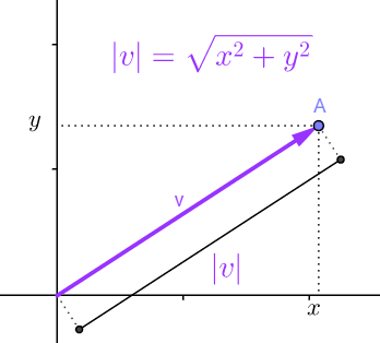
\includegraphics[width = \largurafig]{images/modulo_vetor.jpg}
    }
\caption{Modulo de um vetor.}
\label{fig:modulo}
\end{figure}

\begin{figure}[htbp]
\centerline{
    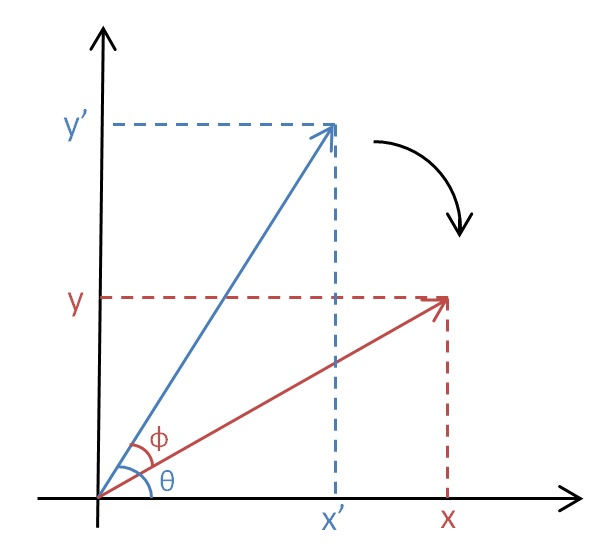
\includegraphics[width = \largurafig]{images/rotação_vetor.png}
    }
\caption{Rotação de um vetor.}
\label{fig:rotacao}
\end{figure}

\subsection{Pushbottons}
A função dos botões de pause e reiniciar está presente no código abaixo. 
Ela foi contruída através de operadores ternários ifs, no qual, na linha 3 se a variável reset for igual a 1,ou seja, se o botão de reset for pressionado, e a variável boleana start for verdadeira a função reset é acionada e o jogo reinicia. Na linha 7, se o botão pause for presionado e a variável start for verdadeira a função pause é acionada e o jogo é pausado. Na linha 10, se a variáveis boleanas constpause e constwin forem verdadeiras e a constmenu for falsa a função printpause é acionada e é impresso na tela o nomenclatura pause. Na linha 14, se a variável constwin for verdadeira a função printwinner é acionada e é impresso o vencedor na tela. Por fim, na linha 16, se a variável constmenu for verdadeira, costwin falso e constpause verdadeiro a função menu é acionado e é impresso na tela o menu do jogo.

\begin{lstlisting}
void Pushbuttons(){
  fill(255);
  if(reset == 1 && start) {
  reset();
      
  }
   if(pause == 1 && start){
      pause();
    }
    if(const_pause && !const_win && !const_menu){
      print_pause();
  }
   
   if(const_win) print_winner();
     
   if(const_menu && !const_win && const_pause) menu();

     
}
\end{lstlisting}
\section{Interfaces do Jogo}
\begin{figure}[htbp]
\centerline{
    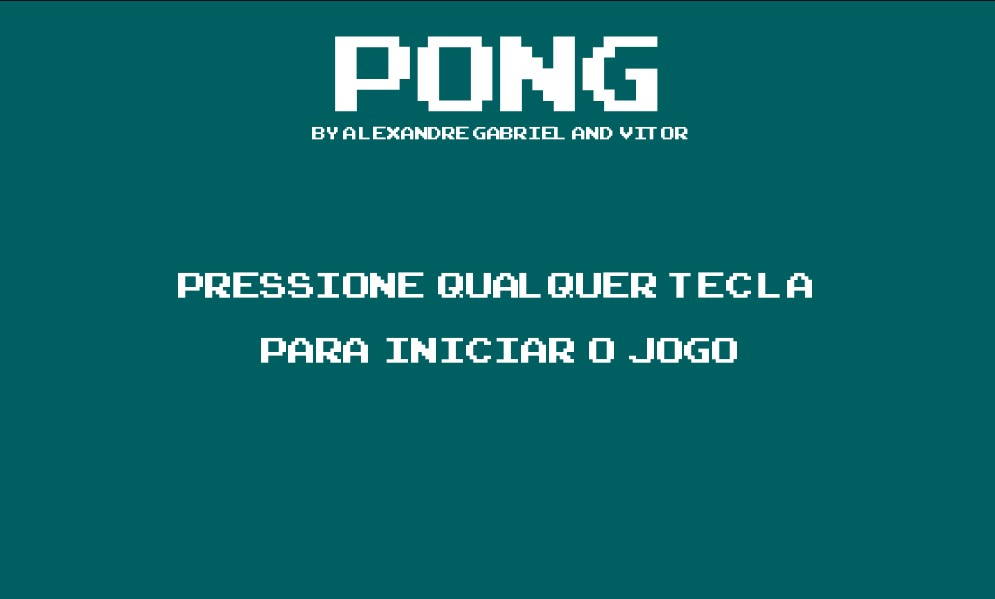
\includegraphics[width= 6cm]{images/Menu.png}
    }
\caption{Menu do Jogo.}
\label{fig:arduino}
\end{figure}
\begin{figure}[htbp]
\centerline{
    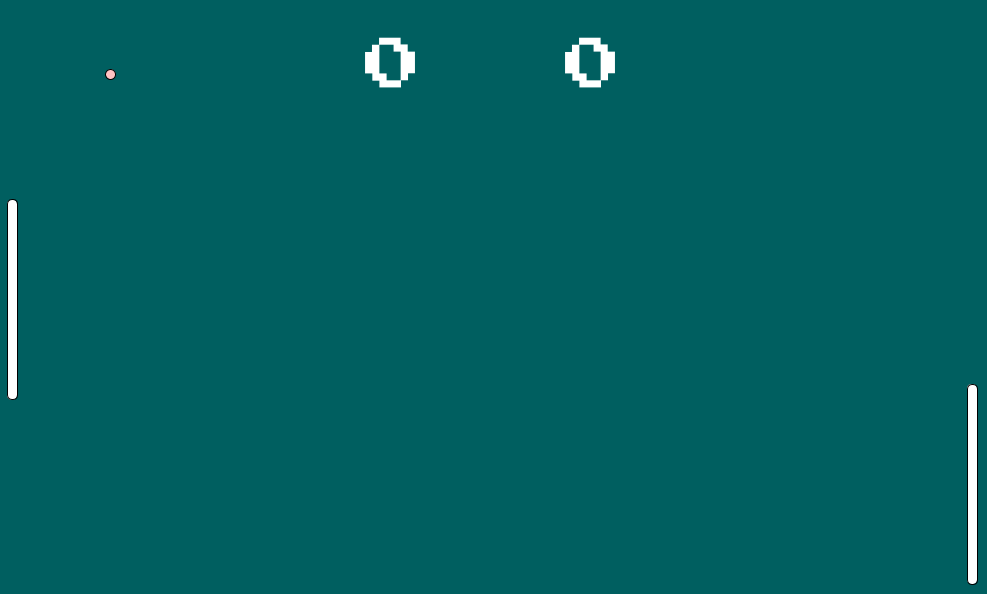
\includegraphics[width= 6cm]{images/Jogo.png}
    }
\caption{Jogo.}
\label{fig:arduino}
\end{figure}
\begin{figure}[htbp]
\centerline{
    
\includegraphics[width= 6cm]{images/Win.png}
    }
\caption{Tela do vencedor.}
\label{fig:arduino}
\end{figure}

\section*{Considerações Finais}
Diante do supracitado,  através do Arduino e seus componentes interligados a IDE Processing foi possível construir o clássico jogo Pong. Dessa maneira, adquiriu-se conhecimentos mais aprofundados da plataforma tornando possível a criação de toda interface gráfica, onde, foi necessária o auxílio da documentação para o entendimento do funcionamento de cada função, que torna a liguagem, baseada em Java, única e acessível até mesmos a profissionais que não são da área como, por exemplo, Designers.

Durante o desenvolvimento do presente projeto também foi possível aplicar os conhecimento adquiridos ao longo da disciplina "Sistemas Embarcados", tais como utilização de sensores e atuadores, leitura de sinais analógicos e digitais, comunicação entre componentes, criação de representações do mundo físico no mundo digital e muitos outros assuntos.

Trabalhos futuros podem contribuir com o projeto de-
senvolvidos por meio da criação de uma placa de circuito impresso para os componente, a fim de evitar possíveis problemas de mal contato ou escape de um dos fios de conexão e tirar o projeto do ambito da prototipacão para uma versão mais robusta e mais próxima de um produto final.
% Sem a linha abaixo o nome "referências" fica muito próximo do texto anterior
\section*{}


%----------------------------------------------------------
\bibliographystyle{IEEEtran}
\bibliography{Bibliography}
%CRITICAL: do not change the above two lines!!!
%----------------------------------------------------------

\end{document}
